\section{Ablation Studies}
\label{app:ablation}
% ============================================================

% We isolate the contribution of the LDM's key design choices across the three experimental regimes of the paper:
% neural-network training-program search, small-molecule design, and antibody CDRH3 design.
These regimes stress different parts of the framework. \texttt{autoresearch} is a \emph{multi-turn code-editing} task: the agent maintains a research state, repeatedly edits a persistent artifact \texttt{train.py}, and can change the representation of the search space as new mechanisms are discovered. Small-molecule and CDRH3 design are closer to \emph{single-step proposal} tasks: at each BO round, the LLM proposes or parameterises a candidate pool, the surrogate acquisition selects from that pool, and the expensive oracle evaluates the selected designs.

The ablations therefore have two complementary purposes. First, in \S\ref{app:abl-pure-llm}, we push the boundary of a pure current-agent research loop on nanoGPT by removing the calibrated BO value entirely. This tests how far an LLM agent can go when it can read its own logs and reflect, but cannot search against a surrogate posterior. Second, in \S\ref{app:abl-ldm}, we keep the value model and study LDM test-time search itself. On nanoGPT this means varying the internal LDM-TTS settings, such as inner search budget, dynamic features, and acquisition choice. On molecules and CDRH3, it means asking whether open-source LLM proposers benefit from larger proposal and acquisition-selection budgets in single-step design rounds.

\subsection{Pure LLM-based research loop}\label{app:abl-pure-llm}

This ablation asks whether the LLM research loop alone is sufficient. Operationally, it is the $\eta=0$ limit of Eq.~\eqref{eq:core}: the agent still reads the history, edits \texttt{train.py}, launches experiments, and keeps improvements, but it does not receive a BO posterior, an acquisition score, or an uncertainty-directed suggestion for what to try next. We deliberately make this a strong LLM-only baseline rather than a straw man: it is meant to push the boundary of what a current advanced agent system can do on this task. The only extra scaffolding is a short reflection instruction that asks the Codex agent to monitor the result log as a whole, ask whether the current iteration verifies the previous hypothesis, extract any new mechanistic insight, and plan the next iteration. This is not human-in-the-loop steering of the scientific direction; it is an end-to-end LLM workflow whose context explicitly asks the agent to behave like a careful experimentalist. Thus the ablation tests the best version of the claim that an LLM, supplied with its own experimental transcript and enough task knowledge to edit the architecture and optimizer, can bootstrap an autonomous research process without an explicit value model.

\begin{figure}[t]
    \centering
    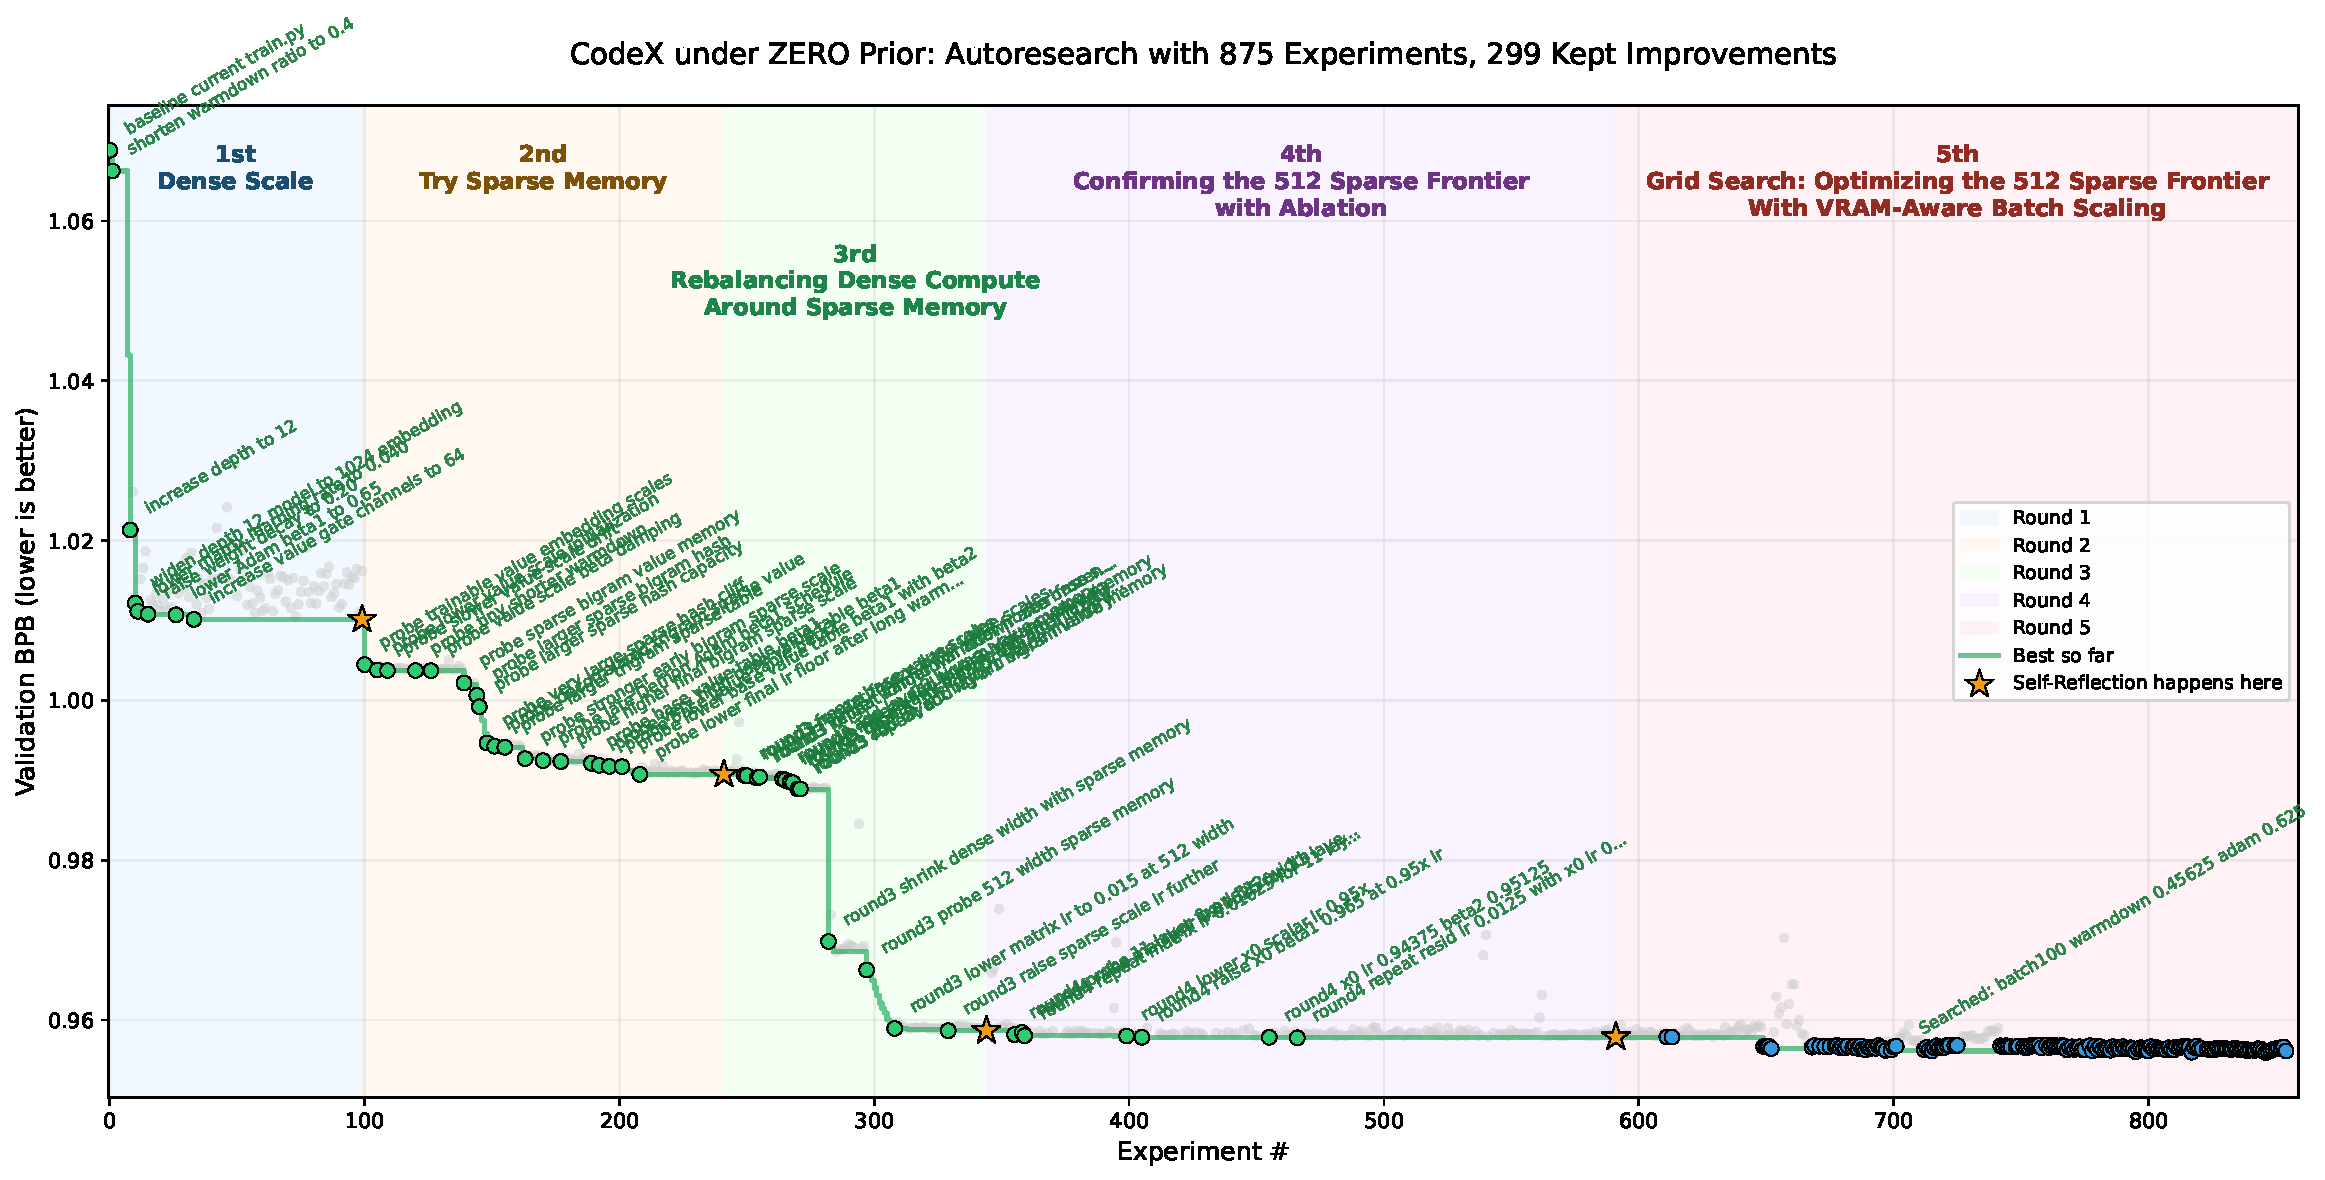
\includegraphics[width=\linewidth]{figure/pure_LLM_autoresearch_progress.pdf}
    \caption{\textbf{Pure LLM research loop on \texttt{autoresearch}.} Validation \texttt{val\_bpb} (lower is better) across $875$ no-BO, no-acquisition experiments. Gray points are individual trials and the green step curve is the best value found so far; yellow stars mark self-reflection checkpoints where the agent summarises the ledger and enters a new research regime. The coloured bands show the loop's staged progress: dense scaling, sparse-memory invention, dense-compute rebalancing around sparse memory, ablation-based confirmation of the $512$-sparse frontier, and final VRAM-aware batch/schedule search. The curve demonstrates that a pure LLM loop can do real sequential research, but also its ceiling: after the large regime shifts it plateaus near $\texttt{val\_bpb}\approx0.956$, above the LDM result of $0.93421$ in Figure~\ref{fig:autoresearch}.}
    \label{fig:abl-pure-llm}
\end{figure}

Figure~\ref{fig:abl-pure-llm} shows that the pure LLM loop is not inert. It discovers several coherent research phases: first dense scaling, then sparse memory, then a rebalance of dense compute around the sparse memory idea, followed by confirmation and grid search around the $512$-sparse frontier. The best-so-far curve falls from the initial $\texttt{val\_bpb}\approx1.069$ to $\approx1.01$ after the first phase, to $\approx0.991$ after the second reflection, and to $\approx0.959$ after the sparse-frontier breakthrough. In other words, a modern code agent with a task-specific prompt and access to its own run log can already produce human-readable, scientifically reasonable progress: it can form hypotheses, translate them into code edits, test them, preserve improvements, and revise its research state.

The archived loop logs show what this ``research work'' consisted of. The agent did not merely enumerate nearby hyperparameters. After each phase it wrote a reflection report: it compressed the ledger into mechanistic claims, labelled memories by regime and mechanism, retrieved positive and negative examples, and used the labelled memories to choose the next experiment family. Table~\ref{tab:pure-llm-trace} summarises the resulting trajectory. The important point is the \emph{statefulness}: the loop changes what it believes the problem is. It begins with ordinary dense scaling, decides that dense capacity has saturated under the five-minute budget, invents sparse associative value memory as a cheaper capacity axis, then shrinks the dense core so that the sparse-memory model can train in time, and finally switches to repeat-first, VRAM-aware frontier tuning once improvements fall into the noise band.

\begin{table}[t]
    \centering
    \footnotesize
    \begin{tabular}{p{0.11\linewidth}p{0.20\linewidth}p{0.37\linewidth}p{0.14\linewidth}}
        \toprule
        Phase & Working hypothesis & Evidence generated by the loop & Best \texttt{val\_bpb} \\
        \midrule
        Dense scaling & Capacity is the early bottleneck, but only while the model can still be trained inside the fixed budget.
        & Depth $10$ and $12$ give large drops; widening the depth-$12$ model helps; depth $14$ worsens near the memory ceiling. The reflection turns this into the rule: dense capacity helps until the update budget becomes the bottleneck.
        & $1.010136$ \\
        Sparse value memory & Dense capacity is saturated, but cheap associative capacity may still help if routed through a bounded value path.
        & Trainable value scales, sparse hashed bigram memory, larger hash tables, decorrelated trigram memory, and phase-specific damping improve the frontier; broader routing and optimizer rewires are recorded as negative memories.
        & $0.990738$ \\
        Dense-compute rebalance & Sparse memory works best when the dense core is smaller and no longer steals the fixed training budget.
        & Causal ablations show trigram memory, early bigram memory, and trainable sparse scales matter. Shrinking dense width to $640$ and then $512$ creates the large breakthrough, after which matrix LR, final LR floor, and sparse-scale LR are retuned.
        & $0.958666$ \\
        Frontier confirmation & The $512$ sparse-memory regime is a narrow compute/update-budget island, and remaining gains require repeats.
        & Widths below and above $512$ lose; removing early ngram memory increases throughput but hurts validation, showing the memory path is causal. Restored-anchor repeats estimate a noise floor of roughly $3$--$5\times10^{-4}$ BPB.
        & $0.957766$ \\
        VRAM-aware batch tuning & Spare VRAM should buy batch/throughput and coupled schedule tuning, not a return to dense scaling.
        & The context retrieves the dense-shrink successes and negative memories against larger dense models, then grid-searches batch size, warmdown, final LR, Adam damping, and weight decay while logging steps, tokens, MFU, and loss slopes.
        & $0.955923$ \\
        \bottomrule
    \end{tabular}
    \caption{\textbf{Mechanistic trace of the pure LLM research loop.} Each row is a phase extracted from the loop logs. The LLM acts like a lightweight experimental scientist: it writes a hypothesis, tests code-level interventions, records both successes and failures, updates a regime label, and carries those memories into the next phase.}
    \label{tab:pure-llm-trace}
\end{table}

This trace is the strongest evidence that the baseline is a genuine research loop. It performs causal ablations (for example, removing trigram memory, early bigram memory, or sparse scales), estimates the noise floor by repeating restored anchors, and eventually augments the ledger with trajectory diagnostics such as steps, tokens, MFU, train/eval gap, and loss slopes. It also learns what not to do: the contexts explicitly retrieve failed routing rewires, failed dense-width probes, crashes, and repeated optimizer mismatches as negative memories. In short, the loop accumulates procedural knowledge, not just a list of winning commits.

The limitation is equally visible. After the third breakthrough, the remaining $\approx500$ experiments are mostly local confirmation and grid search around the same frontier. The loop continues to keep small improvements, but the envelope is nearly flat, ending around $\texttt{val\_bpb}\approx0.956$. This is better than the no-discover Karpathy baseline in Figure~\ref{fig:autoresearch}, which stalls at $0.9767$, but it is still far from the LDM curve, which reaches $0.93421$ under the same H100 five-minute-run setting. The pure LLM loop can reason about its own transcript and name plausible new regimes, but between those reflections it has no calibrated estimate of where improvement is likely, where uncertainty remains high, or when a plateau is evidence that the current boundary is exhausted.

This is the ablation's main conclusion. The bottleneck is not proposal expressivity: the LLM can write useful training code, exploit prior knowledge about how the architecture can be modified, and remember enough of the transcript to pursue multi-stage ideas. The bottleneck is value. Without $\mu_t$, $\sigma_t$, and the acquisition $\acq_t$, \textbf{the run log remains a narrative memory rather than a searchable value landscape}. LDM supplies exactly that missing object: the surrogate turns the same history into a posterior over the program space, and the acquisition turns that posterior into a decision value for both local refinement and boundary-moving discover steps. The pure LLM loop therefore validates the reservoir side of the framework and shows how far current agent systems can already go, while also showing why the BO-value side is necessary for the performance gains in the main experiment.

\subsection{Test-time Search for LDM}
\label{app:abl-ldm}

This ablation asks whether LDM exhibits the same test-time scaling behaviour that motivates inference-time search in language-model reasoning \citep{snell2025scaling}, but in the harder setting where the value is an expensive scientific objective approximated by a surrogate. We keep the outer evaluation budget fixed and vary only the cheap inner-loop budget of LDM-TTS. Concretely, the inner budget has four knobs: (i) how many candidate programmes the LLM proposes at each outer iteration, (ii) how many hypothesis or refinement branches the BO inner loop expands for each candidate before scoring, (iii) how many of those scored candidates the acquisition retains for the next round, and (iv) which acquisition function scores them. The detailed \texttt{autoresearch} test-time-search sweep, with its N4H4/N8H8 budgets and EI vs. posterior-mean comparison, already appears in Section~\ref{sec:ablation-main}; here we keep only the molecule and CDRH3 single-step budget sweeps.

The theory in \S\ref{sec:theory-main} predicts exactly this dependence: increasing the near-acquisition mass available to the tilted sampler reduces the LDM sampling shortfall term, but only if the added candidates are also evaluated by a calibrated value model rather than by language plausibility alone.

\subsubsection{Small-molecule drug discovery}
\label{app:abl-molecule}

The molecular ablation repeats the same question in a chemically open-ended space. Here the expensive evaluation is a two-objective KRAS G12D score, and performance is the dominated Pareto hypervolume under the Vina/activity objectives of \S\ref{sec:cs-molecule-results}. We use the Direct-Softmax LDM pipeline with a Qwen3.5-9B proposer and vary two inner-loop budgets. A label \texttt{proposer}\{K\}\_\texttt{bo}\{M\} means that the LLM proposes a pool of $K$ candidate SMILES strings and the BO/EHVI inner loop is allowed to score up to $M$ candidates and retain the best-scoring ones before the next expensive molecular evaluation is chosen. Thus $K$ controls the breadth of the LLM reservoir draw, while $M$ controls how much of that breadth is exposed to the calibrated multi-objective value.

\begin{figure}[htbp]
    \centering
    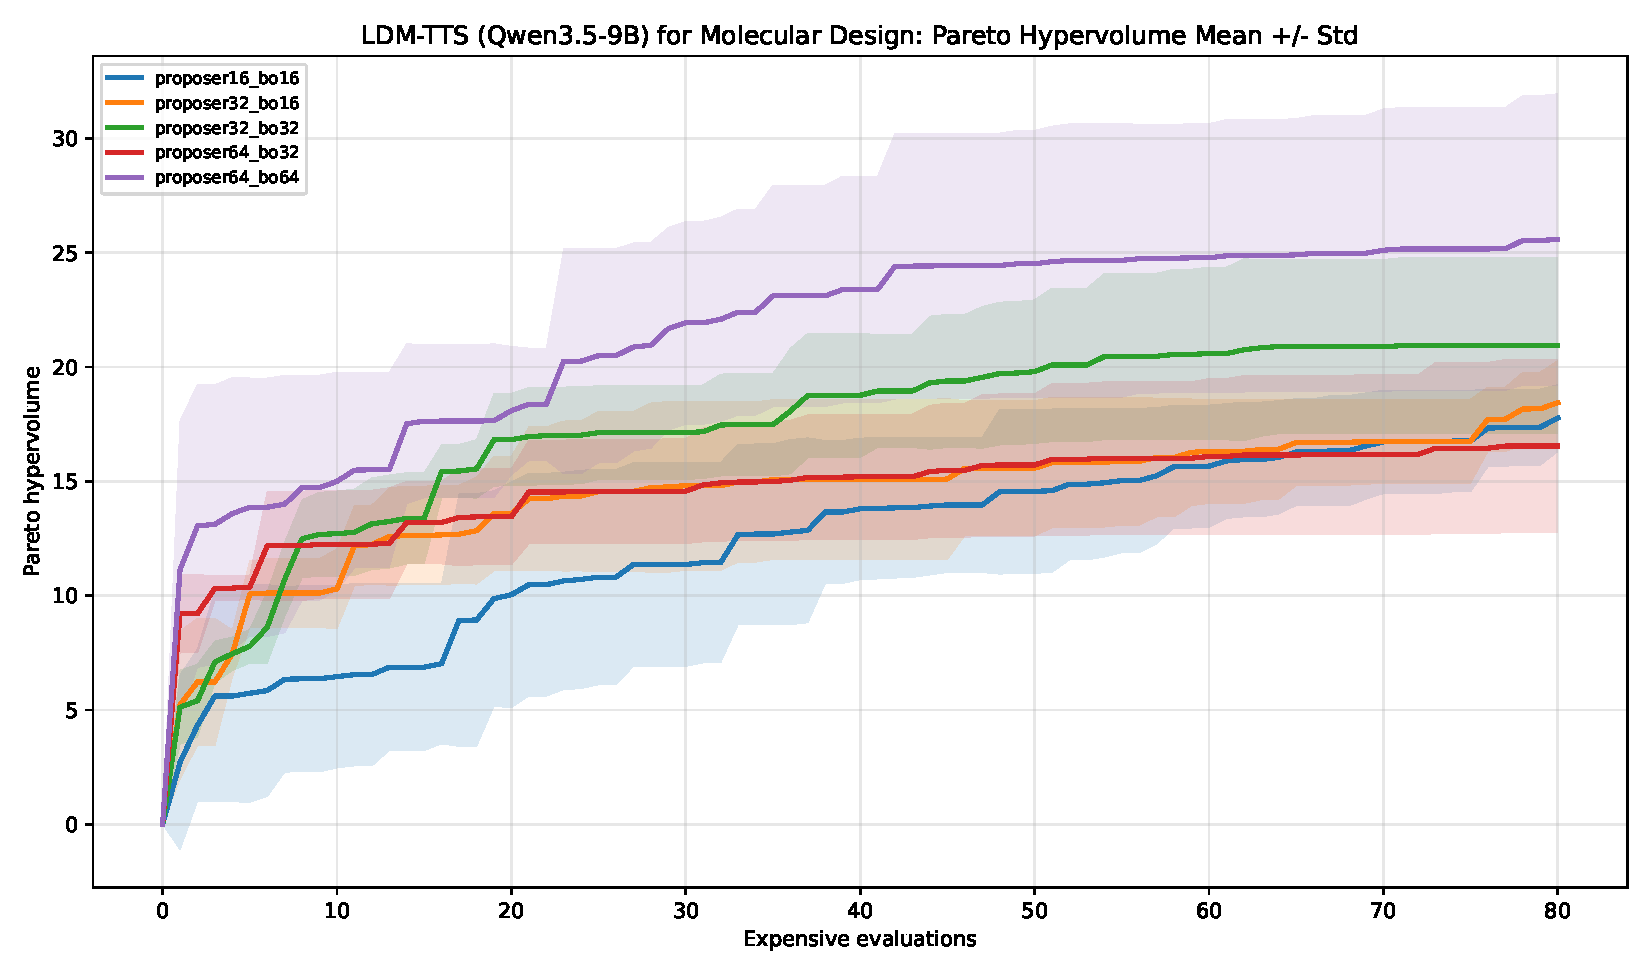
\includegraphics[width=0.8\linewidth]{figure/qwen3_9B_pareto_hypervolume_mean_std.pdf}
    \caption{\textbf{Test-time search scaling for molecular design.} Pareto hypervolume (higher is better) over expensive molecular evaluations for Qwen3.5-9B Direct-Softmax LDM-TTS. Curves show the mean over independent runs, with shaded bands denoting one standard deviation; legend entries report the LLM proposal budget and BO/EHVI acquisition-scoring budget. Balanced scaling of both budgets improves hypervolume most: \texttt{proposer64\_bo64} reaches the strongest final Pareto front, while increasing proposals without matching acquisition bandwidth gives smaller or unstable gains.}
    \label{fig:abl-molecule-tts}
\end{figure}

\begin{figure}[htbp]
    \centering
    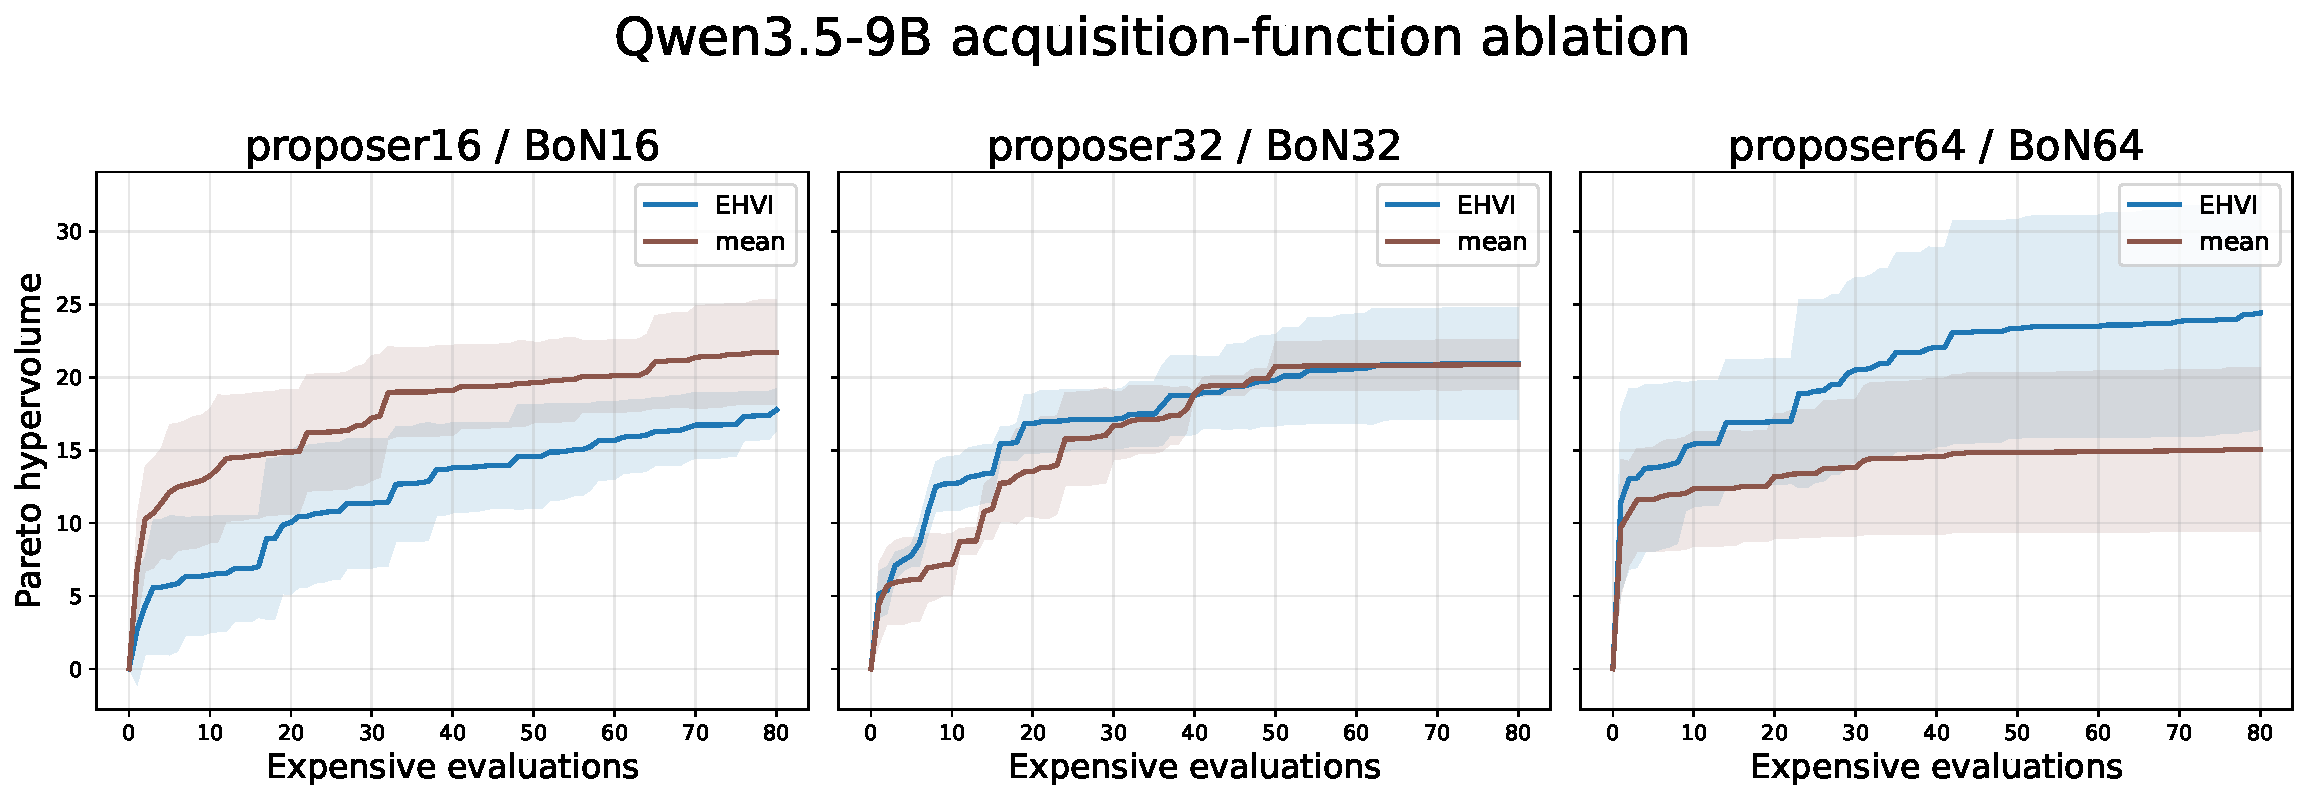
\includegraphics[width=\linewidth]{figure/qwen3_9B_acquisition_ablation_hypervolume.pdf}
    \caption{Abaltion on acquisition function over different search budgets for molecular design.}
    \label{fig:placeholder2}
\end{figure}

Figure~\ref{fig:abl-molecule-tts} shows that test-time compute also scales in the molecular setting, but only when both inner budgets grow together. Increasing the LLM proposal budget from $16$ to $32$ improves the curve, and increasing the BO/EHVI scoring budget from $16$ to $32$ improves it further: \texttt{proposer32\_bo32} dominates the smaller-budget settings through most of the run. \texttt{proposer64\_bo64} makes the largest early jump and keeps the highest final hypervolume; the asymmetric \texttt{proposer64\_bo32} does worse, which shows that broad SMILES generation is useful only when the EHVI side has enough bandwidth to filter the resulting candidates.

Figure~\ref{fig:placeholder2} adds the acquisition-function dimension. At small budgets, mean- or UCB-style acquisitions (a $0.5/0.5$ weighted scalarisation of the Vina and activity objectives) outperform the strict EHVI; as $n$ grows, EHVI overtakes them and continues to improve, while mean-style acquisitions degrade or stagnate. The mechanism is bandwidth: EHVI is built on the strict Pareto frontier and therefore needs a large screening budget to be effective, because multi-objective improvements correspond to sparse non-dominated points. Mean-style acquisitions collapse the two objectives into one scalar, so at small budgets the per-step randomness from a thin screening budget partially substitutes for the missing Pareto signal, smoothing out the optimisation and keeping the curve flat; once the budget grows, EHVI's strict-screening advantage takes over.

\subsubsection{Antibody CDRH3 design}
\label{app:abl-antibody}

% \begin{figure}[t]
%     \centering
%     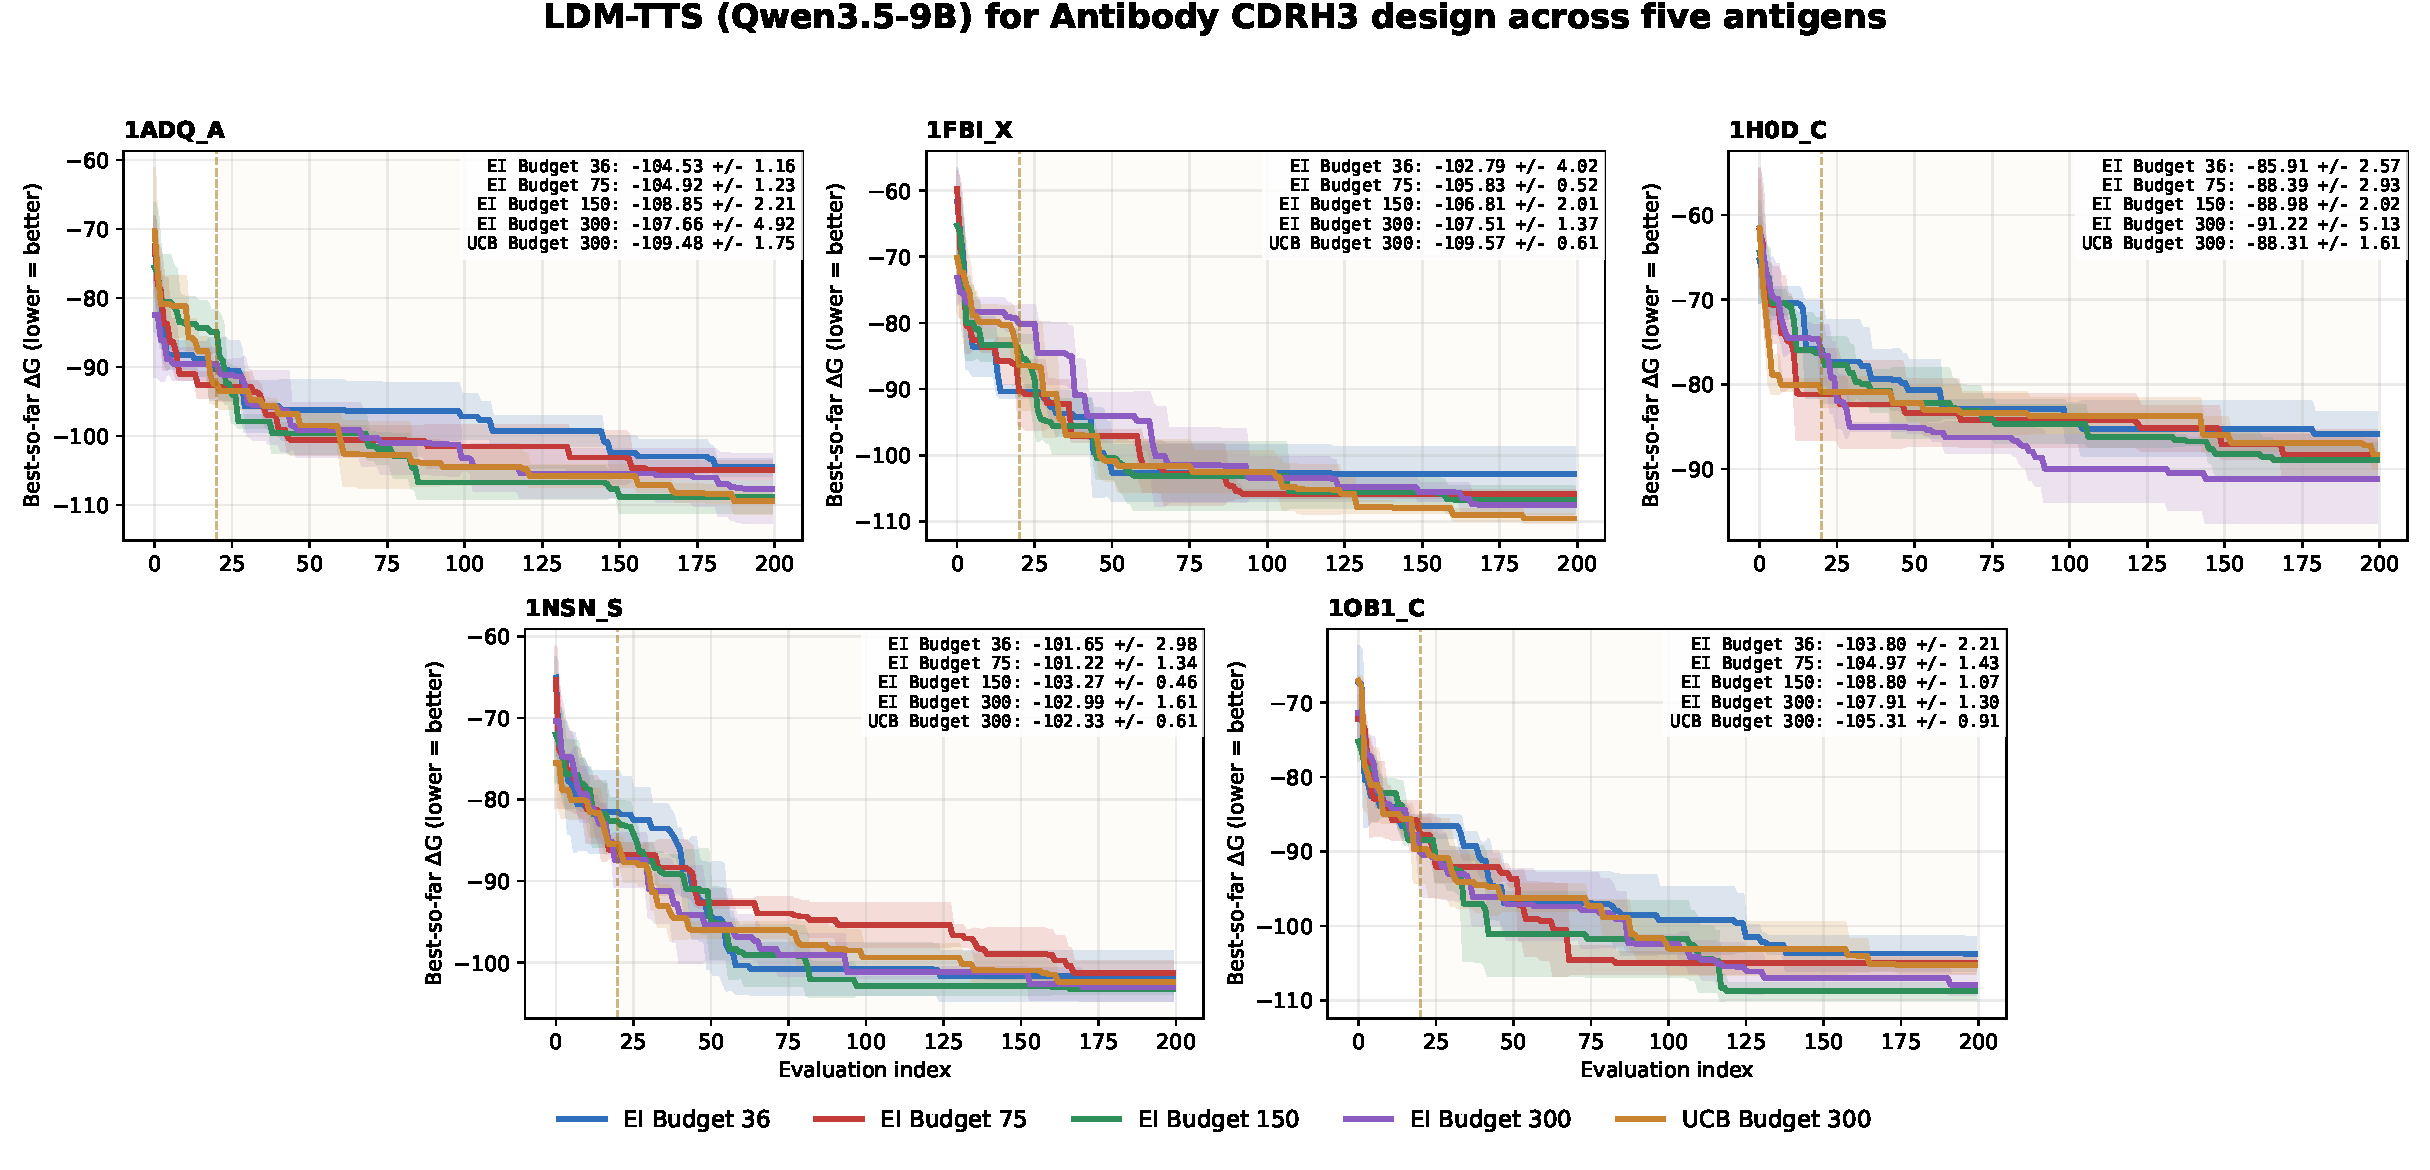
\includegraphics[width=\linewidth]{figure/LDM-TTS-Antigens.pdf}
%     \caption{\textbf{Test-time search scaling for antibody CDRH3 design.} Best-so-far \textsc{Absolut!} binding energy (lower is better) for Qwen3.5-9B LDM-TTS across five antigens. The expensive evaluation budget is fixed at $200$ oracle calls per target. Legend entries vary the LLM proposer budget, i.e., the number of candidate CDRH3 sequences or sequence-neighbourhood samples generated before each oracle query; the BO search budget is not independently tuned and is set to the maximum available number of remaining proposals after filtering. Shaded bands denote one standard deviation across seeds, and panel annotations report the final mean $\pm$ standard deviation. Moderate-to-large proposer budgets improve over the smallest budget on all targets, with the strongest final setting usually occurring at budget $150$ or $300$, showing that additional open-source LLM test-time compute can be converted into better CDRH3 designs when filtered by the BO acquisition.}
%     \label{fig:abl-antigen-tts}
% \end{figure}

% \begin{figure}
%     \centering
%     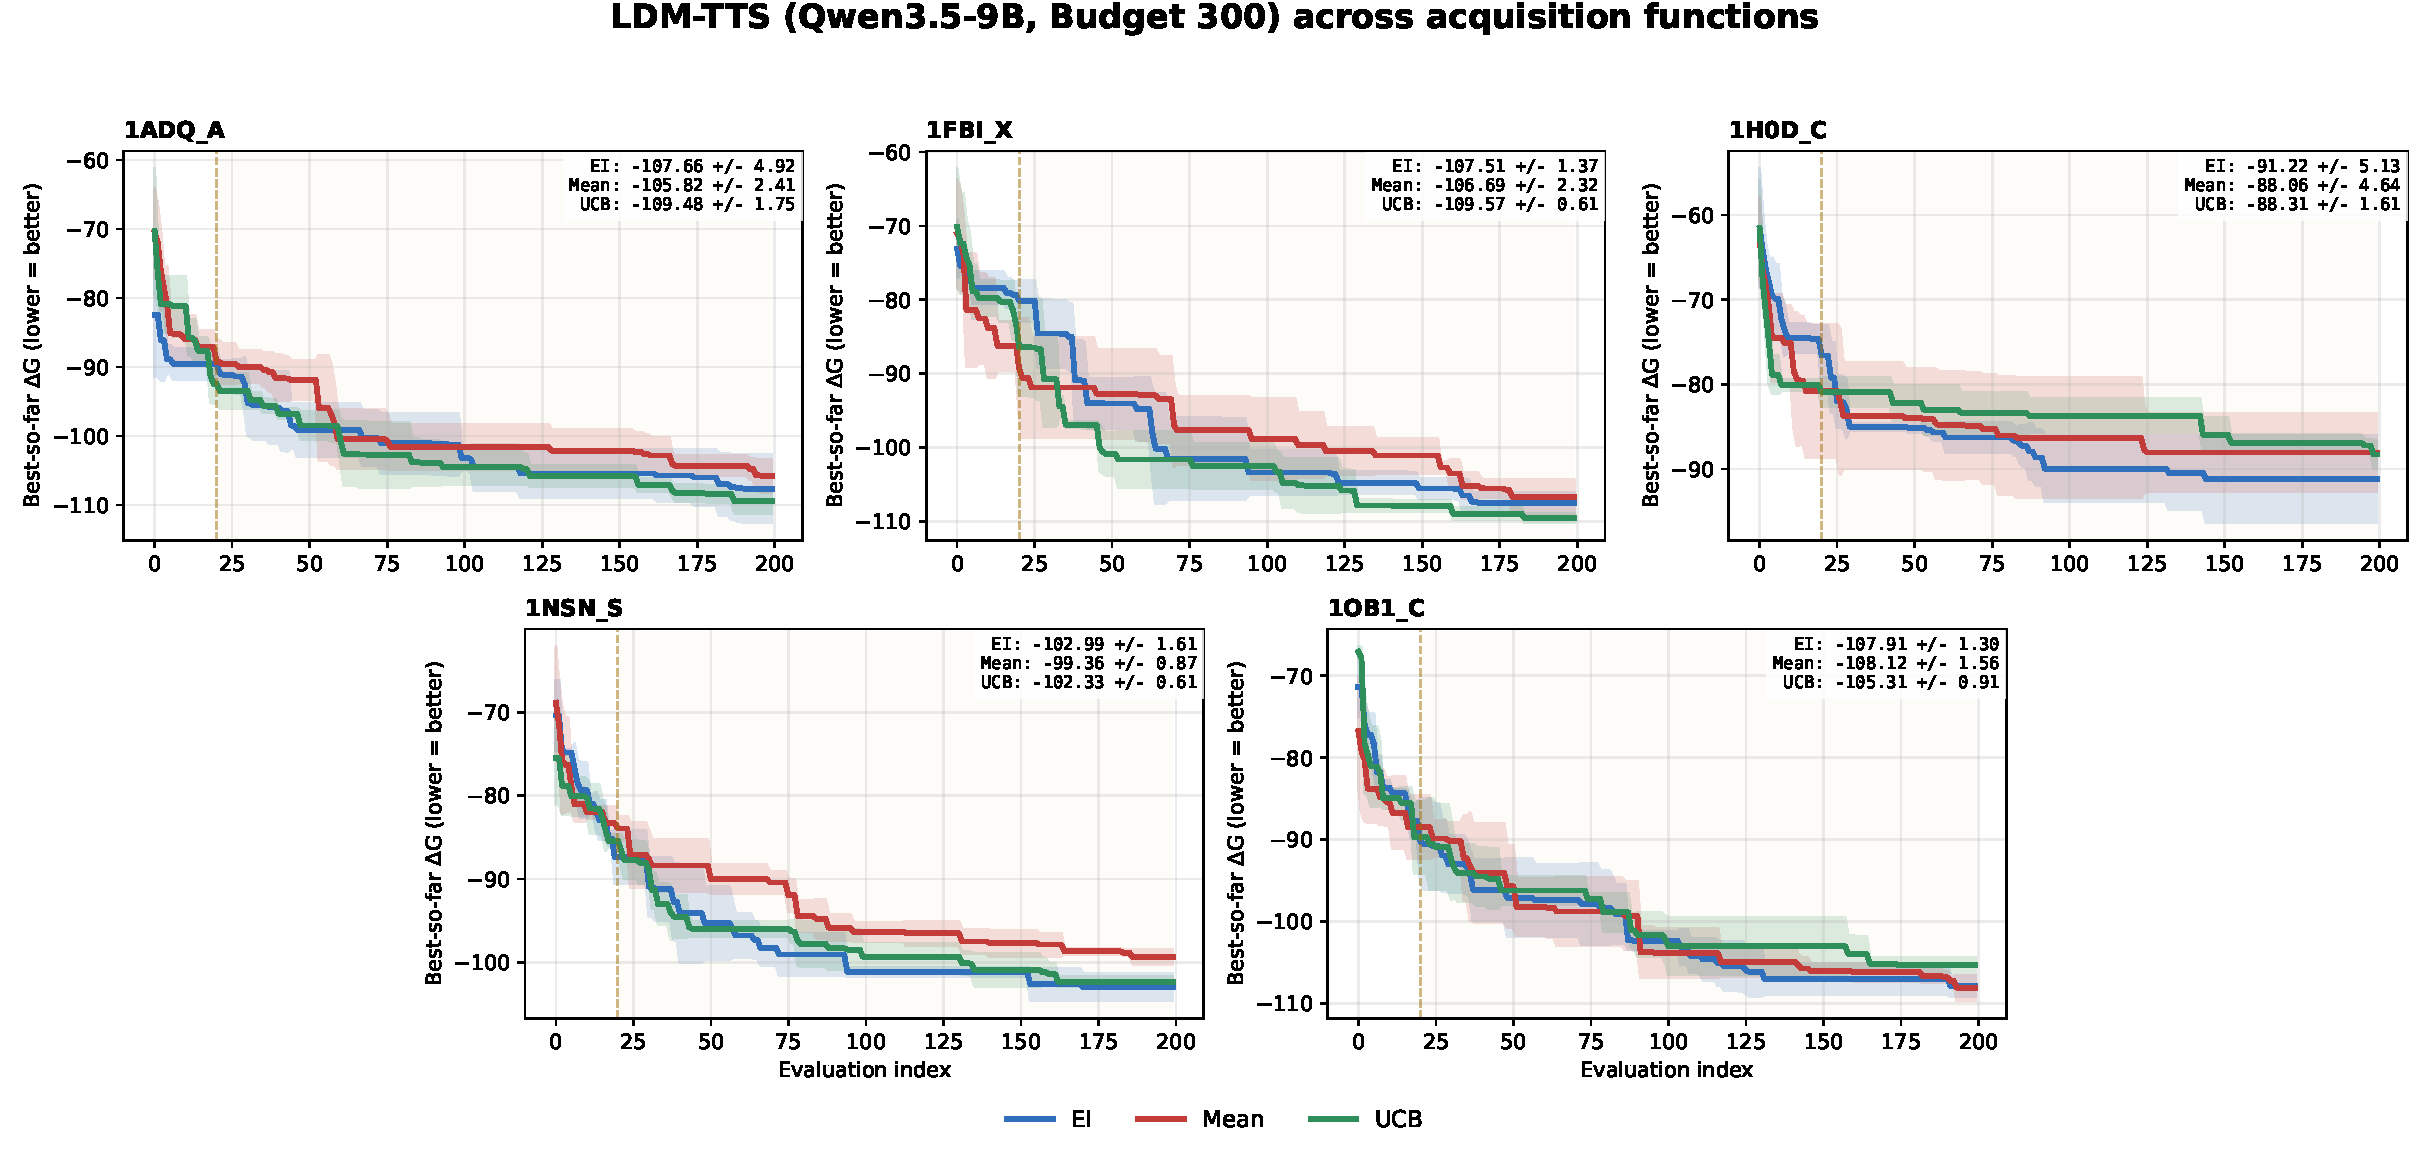
\includegraphics[width=\linewidth]{figure/budget300_acquisition_comparison_5subplots.pdf}
%     \caption{LDM-TTS across acquisition functions}
%     \label{fig:placeholder3}
% \end{figure}

% \begin{figure}
%     \centering
%     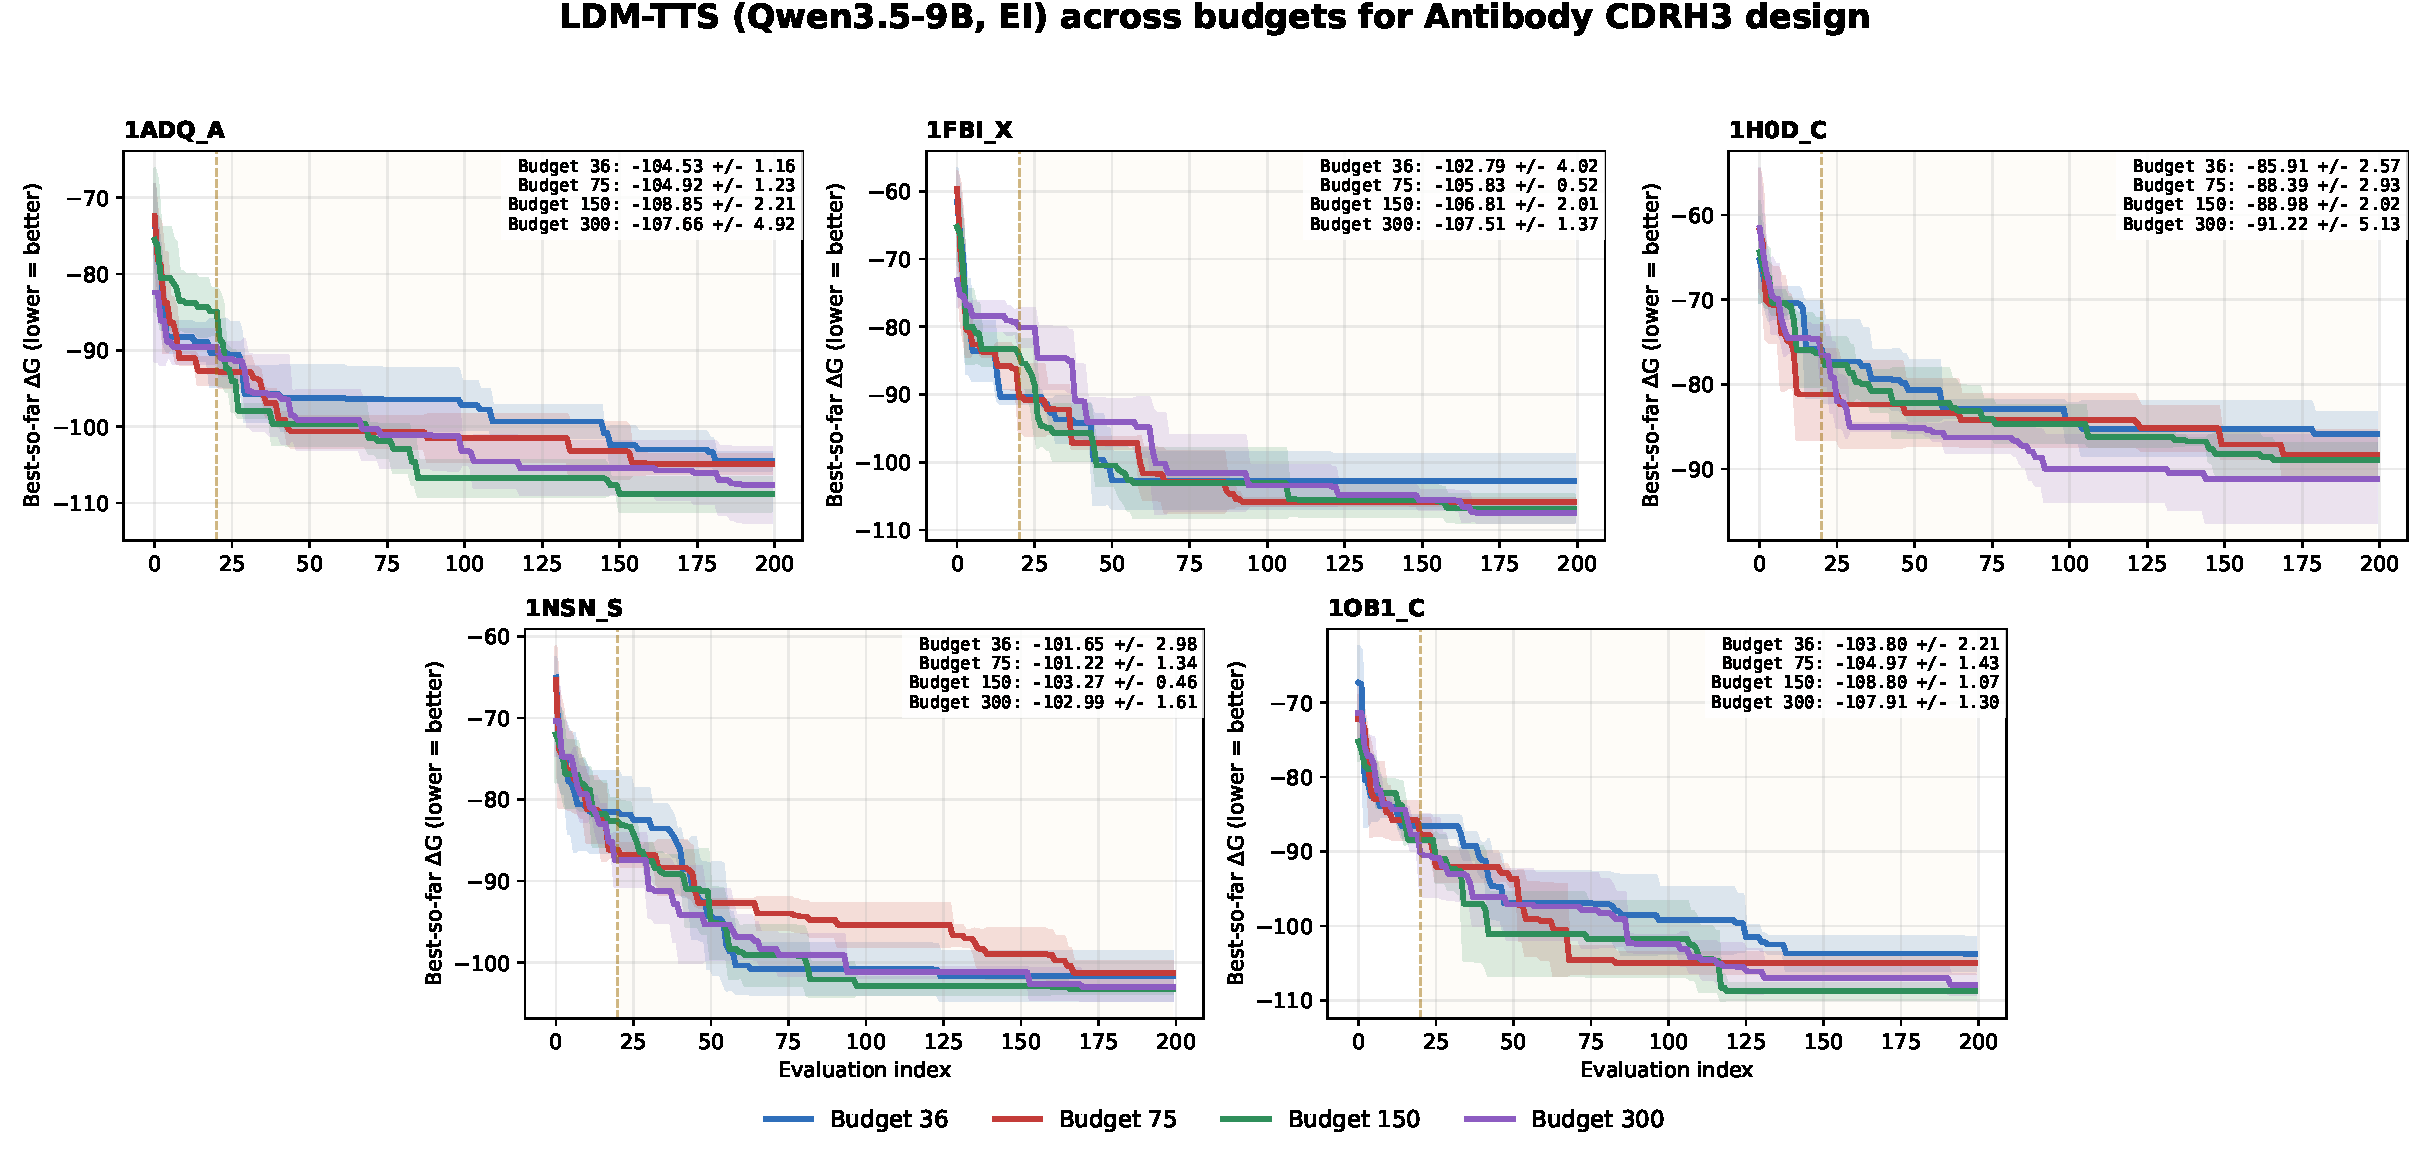
\includegraphics[width=\linewidth]{figure/ei_budget_comparison_5subplots.pdf}
%     \caption{LDM-TTS across budget for Antibody CDRH3 design}
%     \label{fig:placeholder4}
% \end{figure}

\begin{figure}
    \centering
    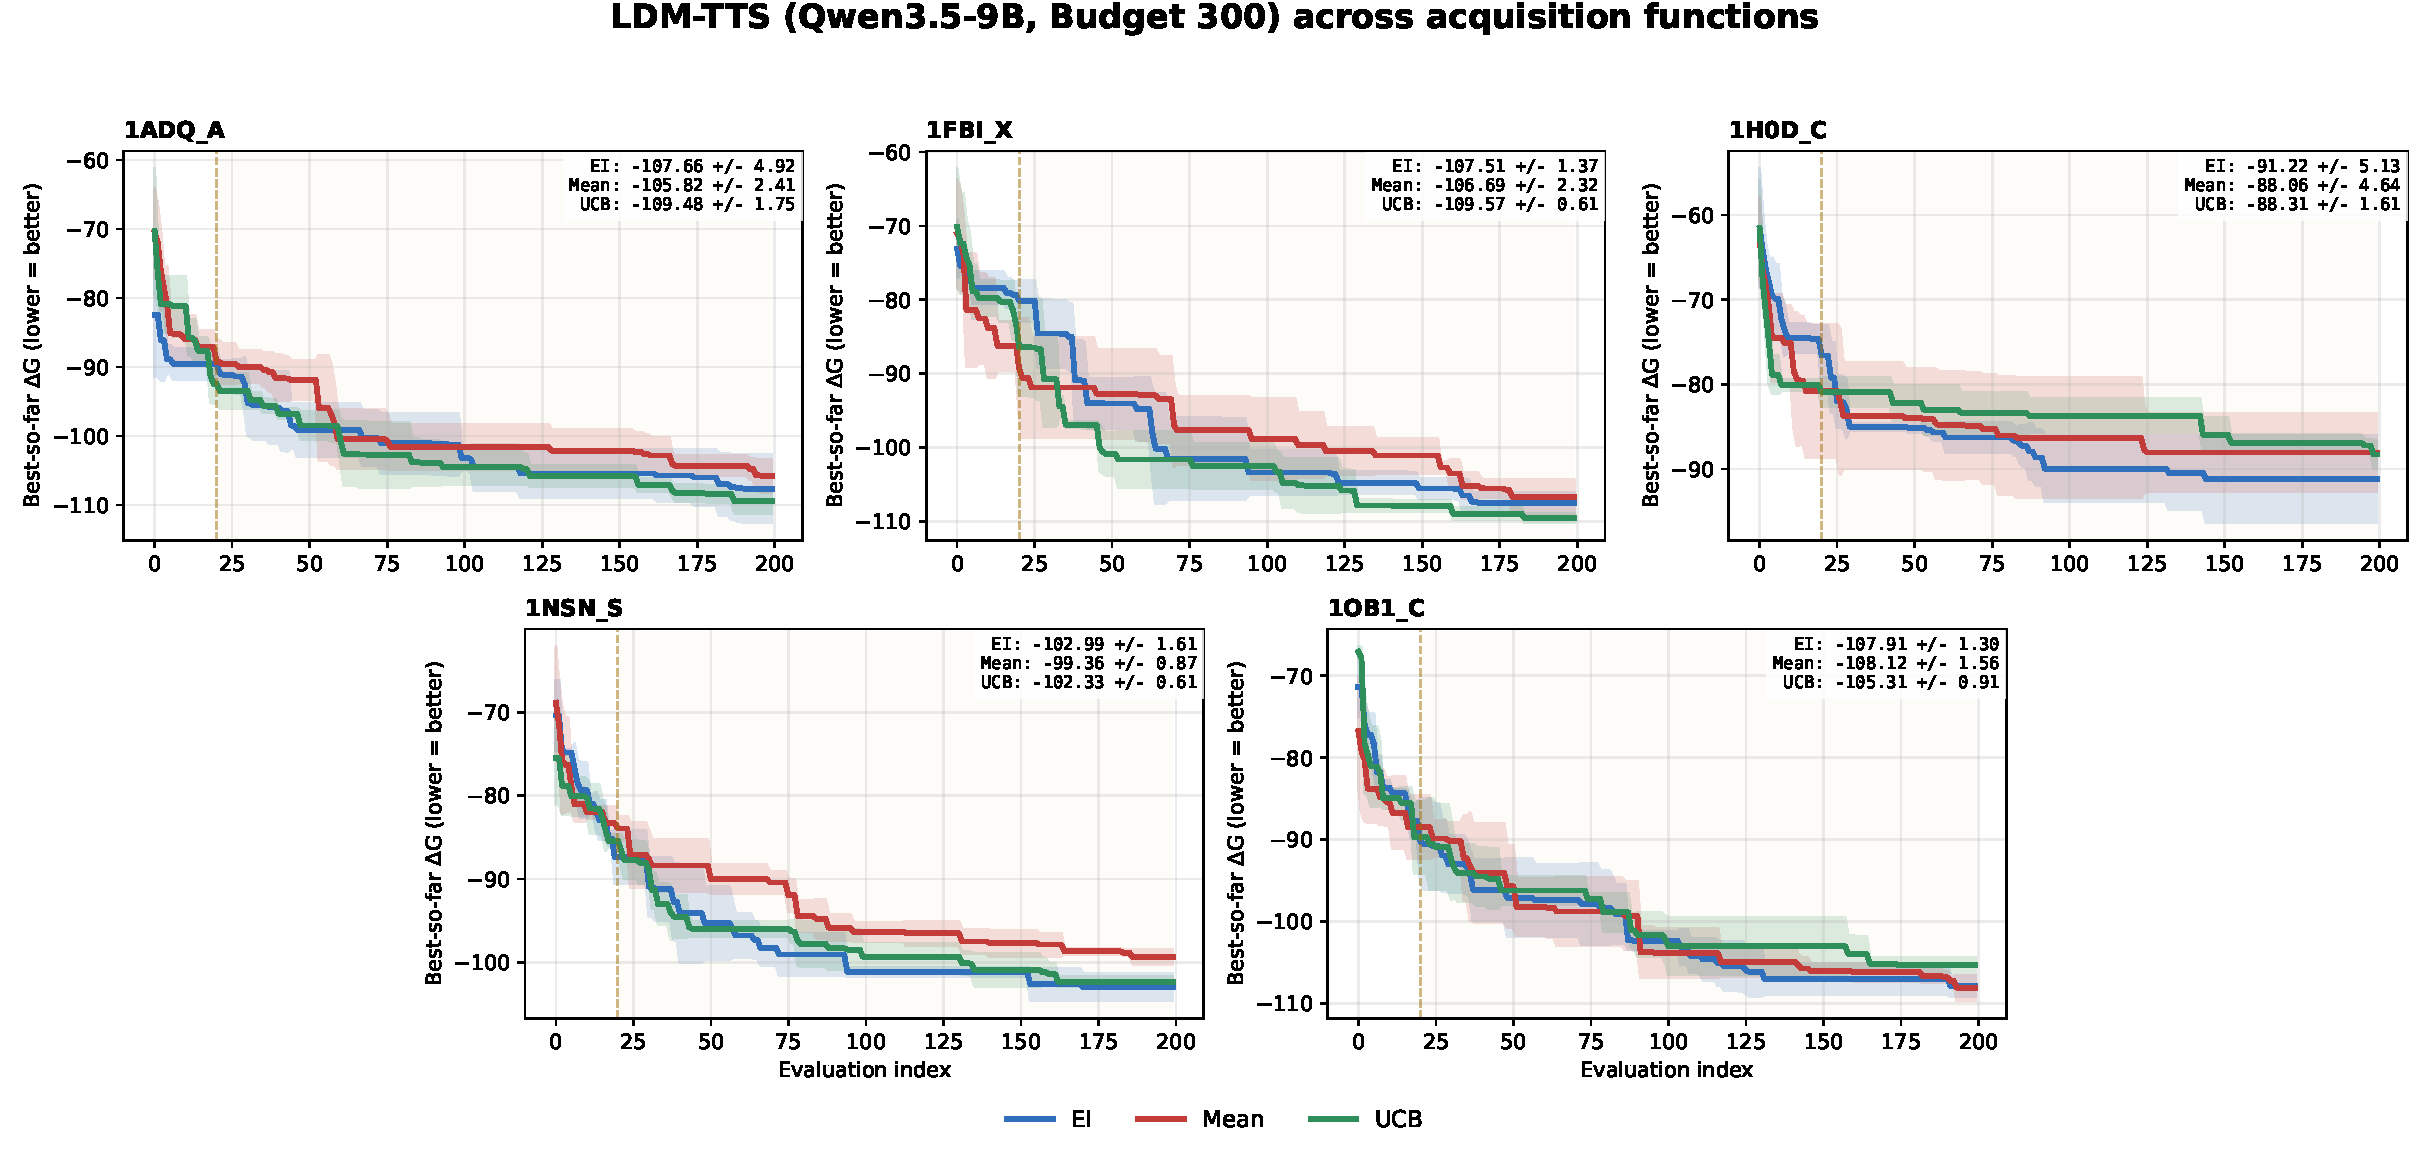
\includegraphics[width=\linewidth]{figure/budget300_acquisition_comparison_5subplots.pdf}
    \caption{Comparison of different acquisition functions for LDM-TTS with a fixed proposer budget of 300 on Antibody CDRH3 design.}
    \label{fig:abl-antigen-acquisition}
\end{figure}

\begin{figure}
    \centering
    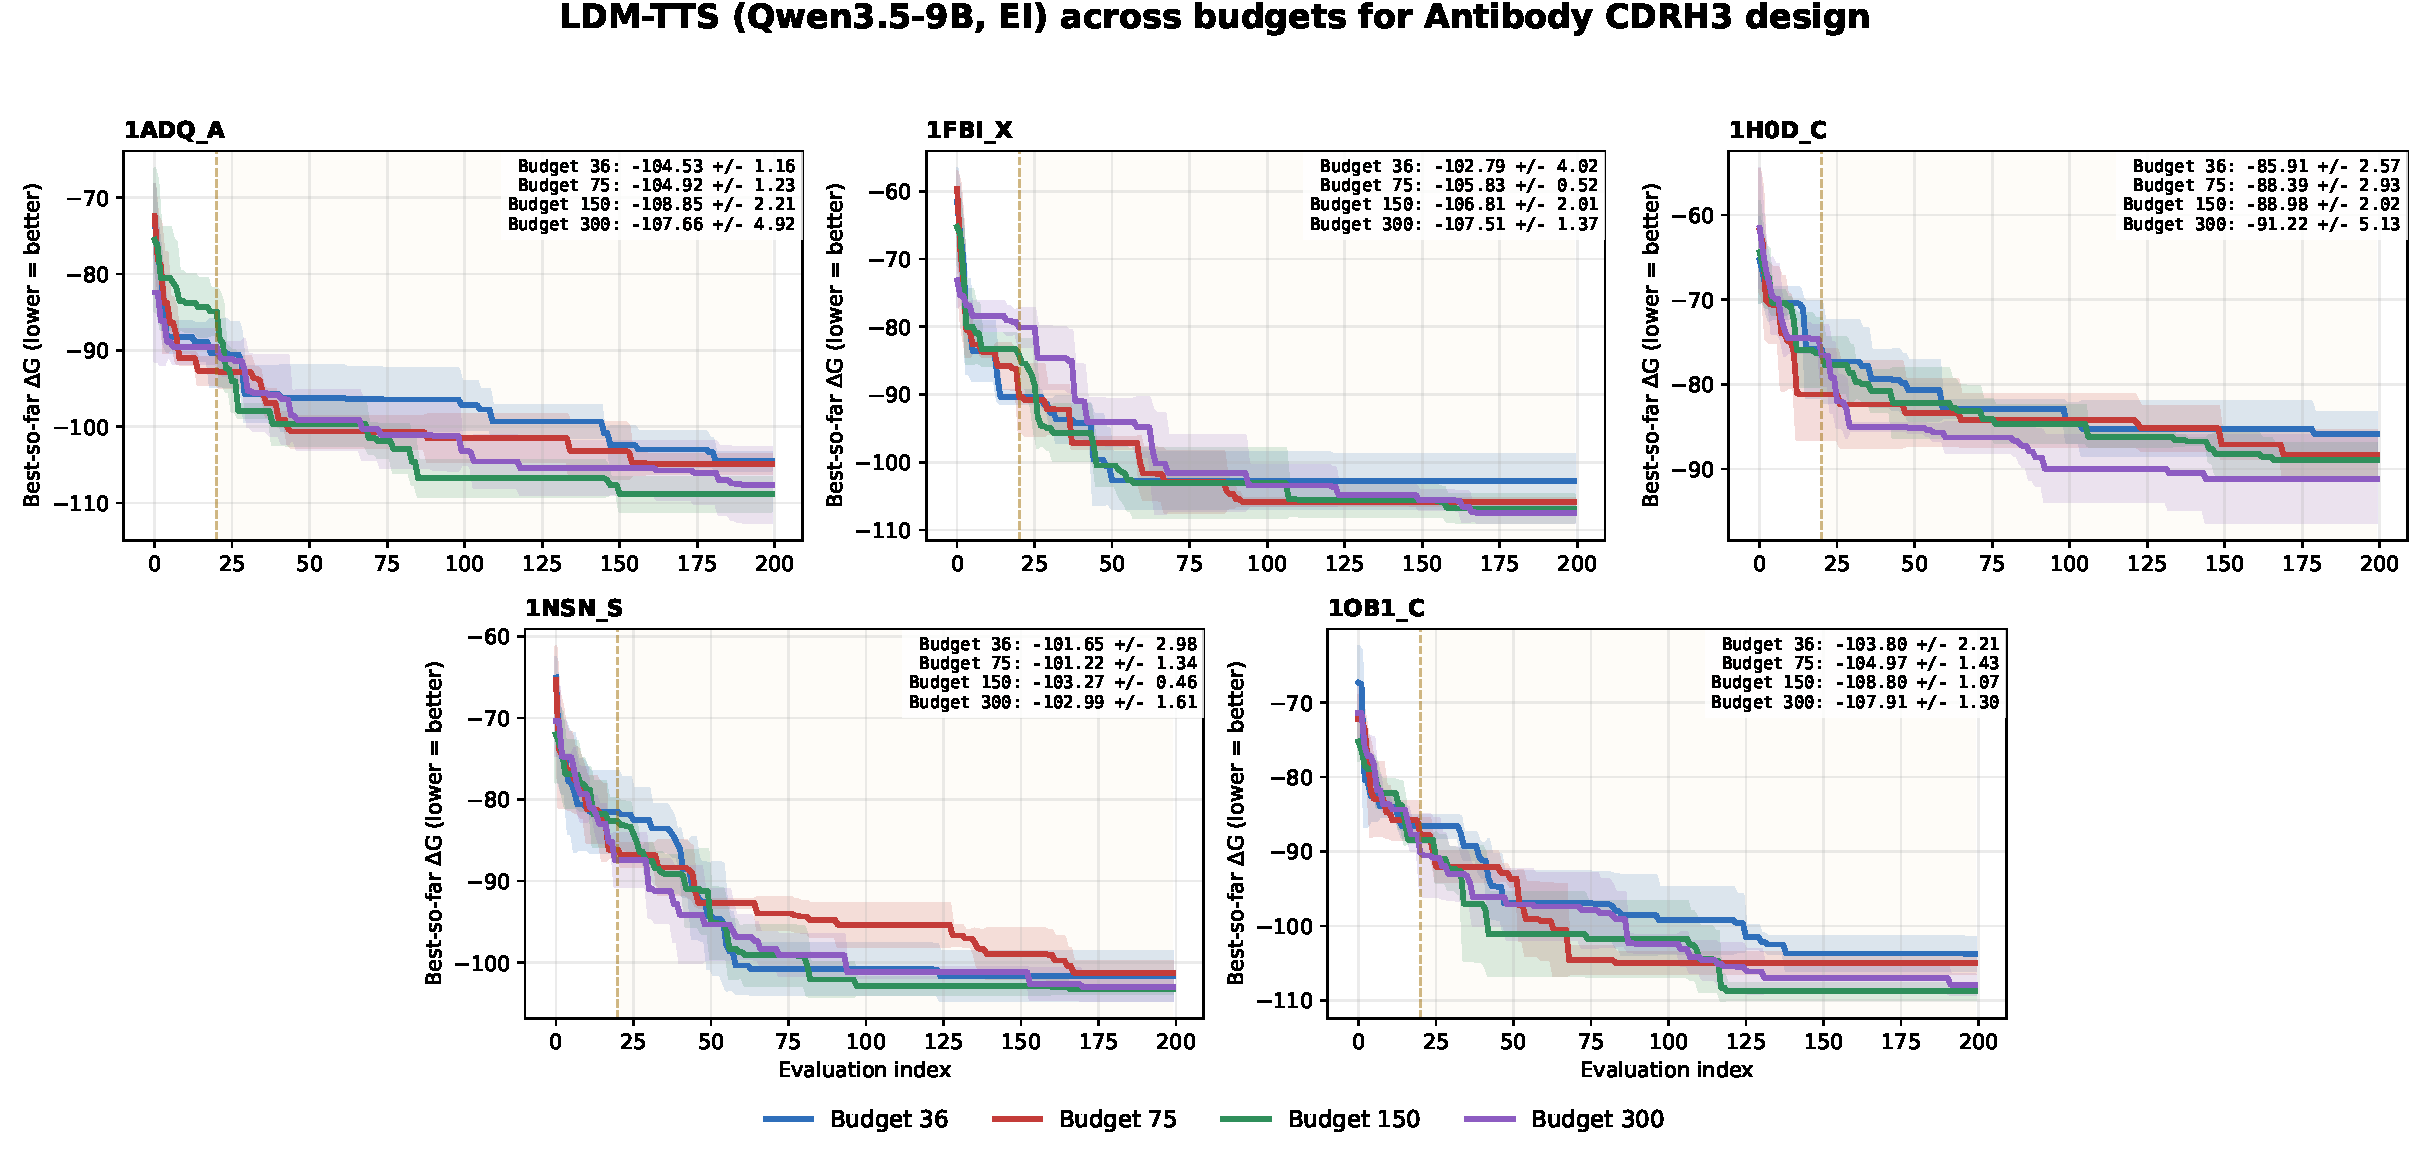
\includegraphics[width=\linewidth]{figure/ei_budget_comparison_5subplots.pdf}
    \caption{Effect of LDM-TTS proposer budget scaling on Antibody CDRH3 design. Each budget denotes the number of candidate sequences or sequence-neighbourhood samples generated before an expensive oracle evaluation. Larger inference-time proposal budgets improve the attainable binding-energy plateau across antigen targets.}
    \label{fig:abl-antigen-tts}
\end{figure}

Figure~\ref{fig:abl-antigen-acquisition} compares different acquisition functions on the five antigens at a fixed proposer budget of $300$. LDM's calibrated acquisitions (EI, UCB and variants) are broadly better than mean-style and random baselines, mirroring the molecular trend above. The result shows that a calibrated acquisition still extracts value from a broader candidate pool even when the open-source LLM has only weak biological priors, and qualifies the §6.5.2 antibody observation: hyperparameter sweeps have only weak sensitivity in this regime, but the choice of acquisition function still matters once the BO side has enough candidates to screen.

The CDRH3 ablation is the sequence-design counterpart of the molecular budget-scaling experiment. The outer oracle budget is again fixed, but here the design space is a known, sparse, discrete sequence space rather than an open-ended SMILES space. We therefore ask a narrower question: does the LDM-TTS proposer budget on its own improve the best sequence found? A label \texttt{Budget} \(N\) denotes an inner proposer budget of \(N\) candidate CDRH3 sequences or neighbourhood samples generated before the next expensive oracle query. The CDRH3 ablation fixes the BO inner-loop side at its maximum feasible setting: after validity checks, deduplication, and history filtering, the acquisition is allowed to score all remaining candidates. So the experiment changes only the cheap LLM-side proposal breadth, not the number of oracle evaluations.

Figure~\ref{fig:abl-antigen-tts} shows the budget effect across antigen landscapes, which is weaker than that observed in molecular design. The smallest budget, \texttt{Budget} $36$, improves quickly at the beginning but usually reaches a higher plateau. Increasing the proposer budget to $75$ already improves the final binding energy on most targets, and the larger $150$ and $300$ budgets give the best final result on all five antigens. The strongest setting is target-dependent: budget $150$ is best on 1ADQ\_A, 1NSN\_S, and 1OB1\_C, while budget $300$ is best on 1FBI\_X and 1H0D\_C. This non-monotonicity is expected in a rugged sequence landscape with finite seeds and a noisy surrogate: after the acquisition has enough candidates to cover the useful local neighbourhoods, further expansion can add redundant or lower-quality regions as well as genuinely novel ones. The main conclusion is therefore not that the largest budget always wins, but that the low-budget regime is systematically acquisition-starved and that moderate-to-large test-time pools substantially lower the attainable binding-energy plateau.

This result complements the main CDRH3 comparison in Figure~\ref{fig:cs-antibody-results}. There, policy-mode LDM outperforms direct token-level generation because the open-source LLM has a weaker biological sequence prior than it has for code or SMILES; emitting a few complete CDRH3 loops does not expose enough useful reservoir mass for BO to exploit. The ablation here isolates what happens once the LDM pipeline can expand the candidate pool: additional inference-time candidates become useful precisely because they are not selected by language plausibility alone. They are filtered by the surrogate acquisition, which converts a larger discrete reservoir into stronger best-so-far binding energy without spending extra oracle calls.

Together, the molecule and CDRH3 ablations show that test-time scaling for single-step design is useful only when the added samples are exposed to a calibrated value model. Richly pretrained SMILES models can absorb large direct proposal batches; sparse biological sequence spaces need enough sequence or neighbourhood coverage before acquisition filtering becomes effective. This complements the nanoGPT ablation: in multi-turn code search, LDM-TTS improves by searching a changing program landscape; in single-step design, it improves by scaling the candidate pool a calibrated acquisition can choose from.

\begin{figure*}[t]
    \centering
    \begin{subfigure}[t]{0.48\textwidth}
        \centering
        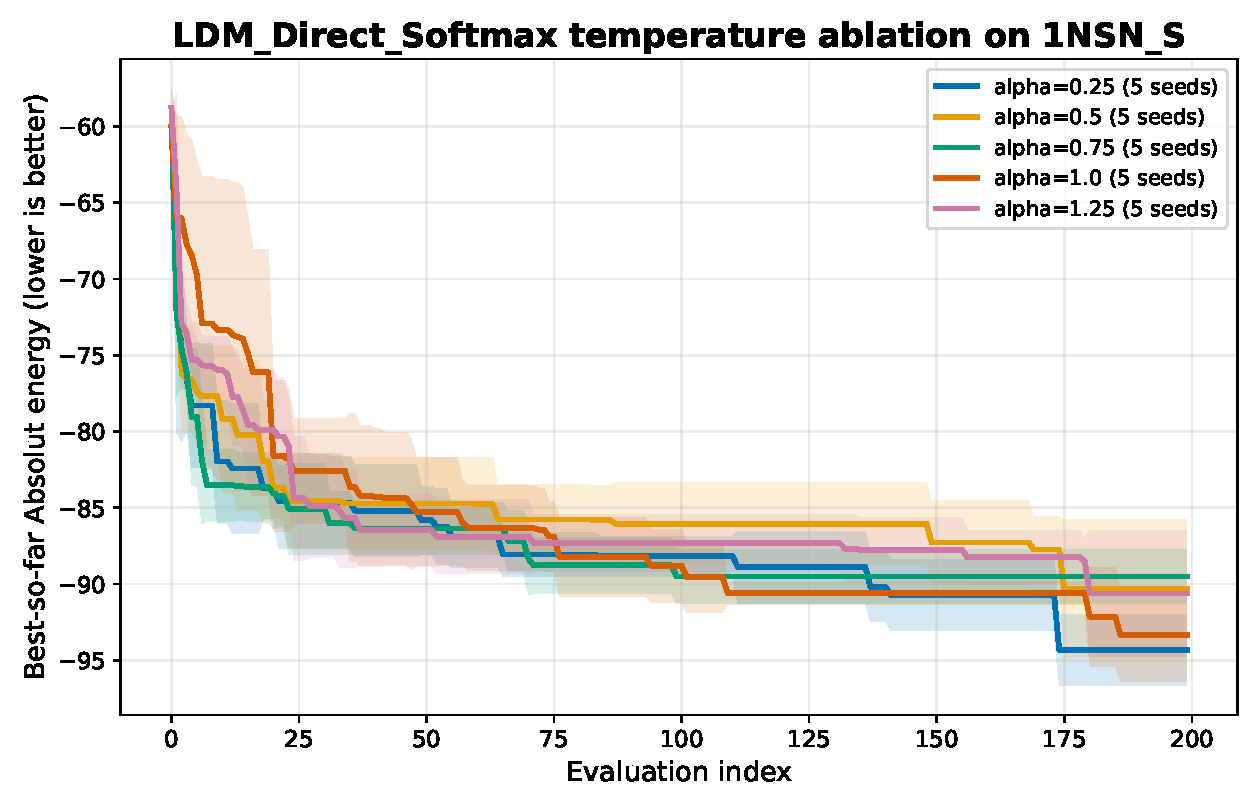
\includegraphics[width=\linewidth]{figure/ldm_direct_softmax_temperature_ablation_1NSN_S.pdf}
        \caption{Effect of the LLM sampling temperature $\alpha$ in LDM\textsubscript{Direct}\textsubscript{Softmax}. The acquisition temperature is fixed to $\eta=1$.}
        \label{fig:ablation-direct-temperature}
    \end{subfigure}
    \hfill
    \begin{subfigure}[t]{0.48\textwidth}
        \centering
        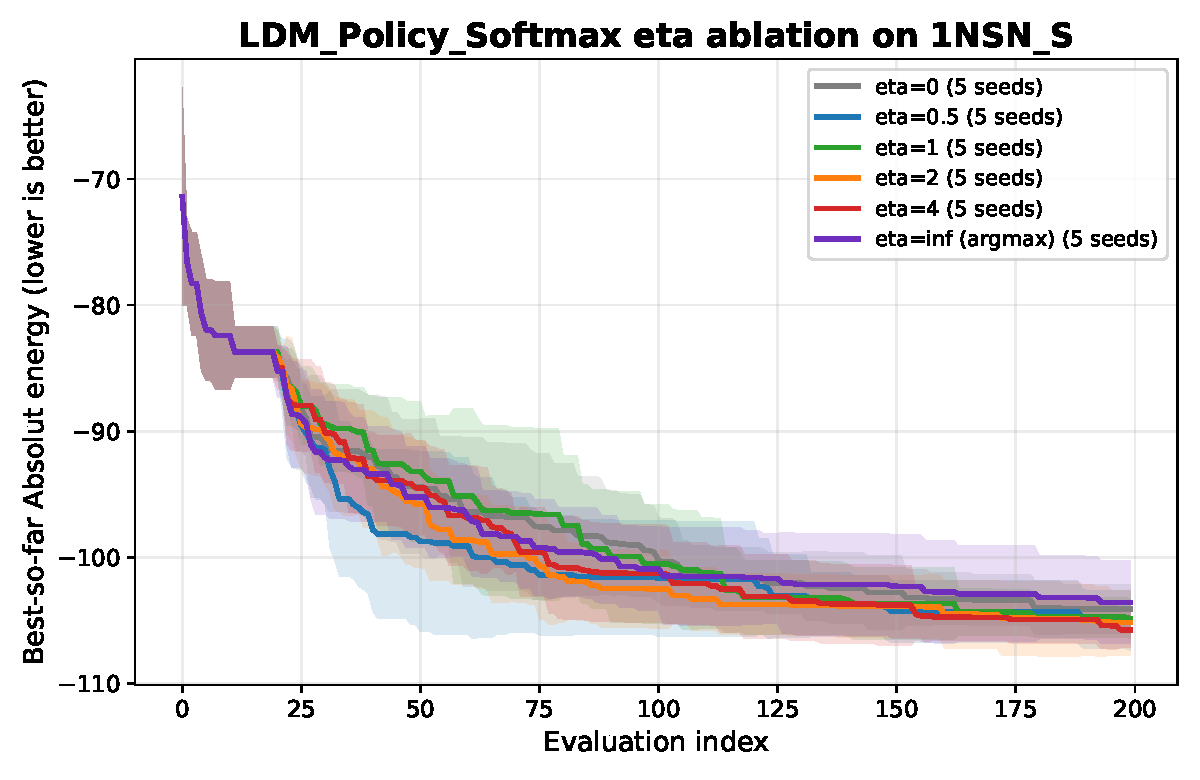
\includegraphics[width=\linewidth]{figure/ldm_policy_softmax_eta_ablation_1NSN_S.pdf}
        \caption{Effect of the acquisition temperature $\eta$ in LDM\textsubscript{Policy}\textsubscript{Softmax}. The LLM sampling temperature is fixed to $\alpha=1$.}
        \label{fig:ablation-policy-eta}
    \end{subfigure}

    \caption{Hyperparameter ablations on the antibody-design task $1\mathrm{NSN\_S}$. Each curve reports the mean best-so-far Absolut energy over five random seeds, with the shaded region showing one standard deviation. Lower values are better.}
    \label{fig:hyperparameter-ablations}
\end{figure*}

\subsection{Hyperparameter ablations for LDM.}
\label{app:abl-hyper-ldm}

We here supplement the sensitivity analysis of the two LDM variants on antigen $1\mathrm{NSN\_S}$ using five random seeds. For LDM\textsubscript{Direct}\textsubscript{Softmax}, we vary the LLM sampling temperature $\alpha\in\{0.25,0.5,0.75,1,1.25\}$ while fixing the acquisition temperature to $\eta=1$. For LDM\textsubscript{Policy}\textsubscript{Softmax}, we fix $\alpha=1$ and vary the acquisition temperature $\eta\in\{0,0.5,1,2,4,\infty\}$. Here, $\eta=0$ corresponds to uniform selection among the policy representatives, while $\eta=\infty$ is equivalent to acquisition-function argmax. The per-temperature curves are plotted in Figure~\ref{fig:hyperparameter-ablations}; we discuss their interpretation below.

This overall behaviour is consistent with the discussion in Section~\ref{sec:ablation-main}. Figure~\ref{fig:hyperparameter-ablations} shows the per-temperature curves. The open-source LLM lacks biological sequence domain priors, so its autoregressive proposals over the $20^{11}$ CDRH3 space are effectively near-random; in the policy variants the LLM already implements an implicit form of acquisition-aware importance sampling by expanding the candidate neighbourhood around promising incumbents rather than committing to a single sequence, which dampens the marginal effect of further reweighting at test time. Consequently, global sweeps over the sampling temperature $\alpha$ and the acquisition temperature $\eta$ on antigen $1\mathrm{NSN\_S}$ produce only weak sensitivity: Direct-Softmax slightly favours low $\alpha$ and Policy-Softmax shows a marginal edge near $\eta=4$, but all error bars overlap. Adjusting the two temperature knobs does not significantly change the final binding energy, which is consistent with the observation in \S\ref{sec:cs-antibody-results} that the policy-mode LDM gain over direct generation comes from the LLM's structural priors rather than from acquisition reweighting alone.